\begin{chapter}{Teoria da Pinça Ótica}
\label{cap2}

\hspace{5 mm}Esse capítulo será dedicado a apresentar teorias que descrevem o aparato de pinça ótica. A ênfase será no modelo Mie-Debye (MD), que foi usado para as simulações e obtenções dos resultados. Outros modelos importantes serão instroduzidos, com a finalidade de gerar uma intuição acerca do assunto. 

Alguns resultados que parecem contra-intuitivos pedem a introdução de alguns efeitos que os explicam. Portanto, a interação de momento angular de spin e orbital do feixe será discutida no contexto da teoria MD, onde a alta abertura numérica da objetiva é a responsável por efeitos de conversão entre os momentos angulares\cite{Bliokh2015}.

\section{Ótica geométrica e limite de Rayleigh}

\hspace{5 mm}Uma forma intuitiva de entender o aprisionamento ótico de objetos esféricos e transparentes é no regime em que estes possuem um raio muito maior que o comprimento de onda do feixe incidente. Este limite é chamado de ótica geométrica, ou ótica de raios, no qual feixes podem ser tratados de forma geométrica definindo-se sua trajetória.

Por outro lado, no limite em que o raio é muito menor que o comprimento de onda, temos o limite de Rayleigh, em que nós podemos aproximar a microesfera por um dipolo elétrico.

O feixe presente em uma pinça ótica tem a forma de um cone sólido com um perfil de intensidade radial. Nessa explicação, vamos olhar o comportamento de uma casca desse cone sólido com angulo de abertura $\theta$ fixo. Dependendo de como os vetores de momento $p$ diametralmente opostos mudarão ao passar pela esfera, podemos inferir a força que ela sofrerá pela variação dos pares desses vetores. Como só estamos interessados em ver o comportamento de aprisionamento da esfera pelo feixe, vamos ignorar efeitos de absorção e reflexão. 

Começamos pelo caso mais simples: quando a ponta da casca do cone, ou a posição focal do feixe, coincide com o centro da esfera (figura \ref{foco_coinc}). Nesse caso, o ângulo de incidência dos raios é normal a superfície da esfera, e o ângulo de transmissão é igual ao de incidência pela lei de Snell.
%
\begin{figure}[h]
\begin{center}
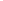
\includegraphics[scale=.8]{geom_foco_coincII}
\caption{Foco coincidente ao centro da esfera. Essa corresponde a posição de equilíbrio estável da esfera.}
\label{foco_coinc}
\end{center}
\end{figure}
%
Assim como ao entrar na esfera, o raio que sai da esfera também incide normalmente à superfície de dentro. Não há mudança na direção do vetor momento, e portanto não há força sendo exercida na esfera. Por simetria, não esperamos que as outras componentes do cone sólido façam força na esfera.

Quando deslocamos a posição do foco em relação ao centro da microesfera, a lei de Snell preve que os raios serão refratados. Começamos deslocando na direção axial, ou seja, com o centro da esfera no eixo do cone (figura \ref{foco_axial}).
%
\begin{figure}[h]
\begin{center}
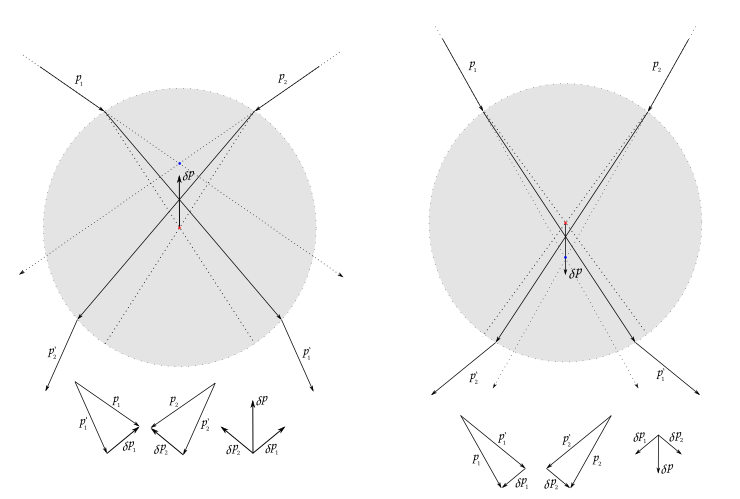
\includegraphics[scale=.8]{geom_foco_axialII}
\caption{Centro da microesfera (ponto vermelho) no eixo do cone, acima (esquerda) e abaixo (direita) da posição do foco (ponto azul). O momento que a esfera adquire ${\mathbf\delta P}$ é $-({\mathbf \it P'}-{\mathbf \it P}$), que é menos a variação de momento do campo, por conservação.}
\label{foco_axial}
\end{center}
\end{figure}

De forma análoga ao caso anterior, ao deslocar verticalmente o foco em relação ao centro da esfera, o momento que a esfera recebe do feixe aponta para o centro deste.
%
\begin{figure}[h]
\begin{center}
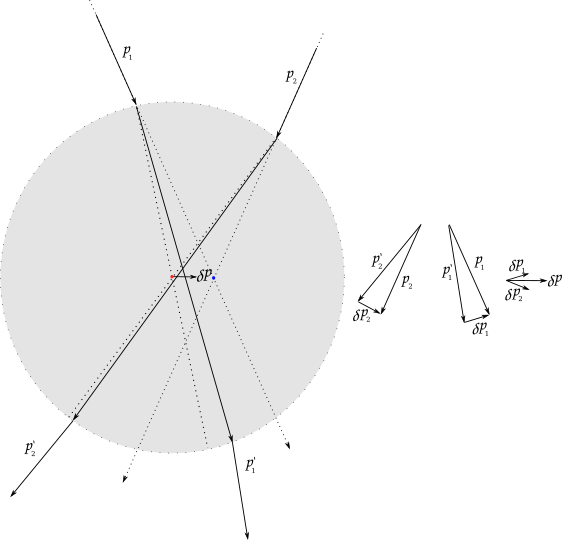
\includegraphics[scale=.7]{geom_lateralIII}
\caption{Centro de massa da microesfera ganha momento na direção do foco do feixe.}
\label{foco_lateral}
\end{center}
\end{figure}
%

Para os casos em que há reflexão e absorção, o efeito resultante é sempre uma força na direção da propagação do feixe. O motivo é que feixes que são refletidos têm sua componente de momento perpendicular à superfície reflexora invertidas. Por conservação de momento, a esfera ganha o dobro de momento nessa direção. No caso da absorção é ainda mais simples: a esfera ganha todo o momento da parte do feixe absorvido.

No caso em que a microesfera é muito menor que o comprimento de onda, chamado limite Rayleigh, podemos aproximar o centro espalhador por um dipolo induzido pelo campo. Dessa forma, a força no dipolo ${\mathbf p}$ será dada por \cite{Mazolli}:
%
\begin{equation}
{\mathbf F} = \nabla({\mathbf p}\cdot{\mathbf E}),
\end{equation}
%
com ${\mathbf p}$ sendo dado por \cite{Jackson1998}:
%
\begin{equation}
{\mathbf p} = 4\pi\epsilon_0 \frac{\epsilon-1}{\epsilon-2}a^3{\mathbf E}.
\end{equation}
%

Podemos concluir que a força vai ser proporcional a ${\mathbf E}^2$, que é proporcional por sua vez à intensidade do campo. Se ${\mathbf E}$ e ${\mathbf p}$ têm o mesmo sentido, a força apontará sempre para a região de maior intensidade. Isso ocorre desde que $\epsilon>1$. Essa é a força que chamamos de força de gradiente.

\section{Modelo Mie-Debye}
\label{MD}

\hspace{5 mm}Discutiremos brevemente nesse capítulo o modelo MDSA+. Para entender a orígem das expressões para a força, vamos começar do problema mais simples. Trataremos nessa seção as bases do modelo Mie-Debye, para uma onda de polarização circular (direita ou esquerda). Os detalhes de tais cálculos podem ser encontrados em \cite{Mazolli}, e não estarão no presente trabalho para evitar repetição. 

Começamos pela forma como se faz o cálculo da força em uma amostra na pinça ótica \cite{Jackson1998}:

\begin{equation}
\vec{F} = \oint_{\sigma} \hat{n} \cdot T d \sigma - \mu \epsilon \frac{d}{dt} \int_{\nu} \vec{S} d \nu,
\label{2_F}
\end{equation}

onde $\sigma$ é uma superfície que envolve a amostra na pinça ótica, $\nu$ é o interior dessa superfície, $T$ é o tensor das tensões de Maxwell e $\mu$ e $\epsilon$ são a permeabilidade magnética e a permissividade elétrica do meio envolvendo a amostra, respectivamente. 

O primeiro passo, portanto, é calcular o campo eletromagnético incidente e espalhado nessa amostra (centro espalhador). O campo incidente na amostra tem formato cônico sólido, gerado pela objetiva. Montaremos esse campo superpondo ondas planas. Para tanto, começamos tratando do caso de uma onda plana se propagando na direção $z$, com polarização circular. Essa é a polarização conveniente para expansão do campo em multipolo (ondas esféricas ou ondas parciais). Outros casos de polarização serão discutidos adiante. 

A base de multipolos é a ideal para problemas com simetria esférica, pois são compostas pelos harmônicos esféricos na parte radial, que são autofunções dos operadores de momento angular $L^2$ e $L_z$. Esse fato será importante para obter os campos vetoriais a partir dos potenciais de Debye, que serão definidos a seguir: 

\begin{equation}
\Pi^{E}=\sum\limits_{J} \Pi^{E}_J=\sum\limits_{J}\frac{ ({\mathbf r}\cdot{\mathbf E })_J }{J(J+1)} \qquad e\qquad \Pi^{M}=\sum\limits_{J} \Pi^{M}_J=\sum\limits_{J}\frac{ ({\mathbf r}\cdot{\mathbf H })_J }{J(J+1)} .
\label{debye_def}
\end{equation}
%
com

\begin{equation}
{\mathbf E}=E_0(\hat{x}\pm i \hat{y})e^{ikz-i\omega t} \qquad e\qquad {\mathbf H}=\frac{n_1}{\mu c}(\mp i){\mathbf E}.
\label{onda_plana}
\end{equation}
%
onde $n_1$ é o índice de refração do meio ao redor da amostra, $k$  e $\omega$ são o vetor de onda e a frequência angular do feixe, sendo $\omega/k=c$ a velocidade da luz no vácuo. Tais potenciais serão úteis para resolver o problem do espalhamento Mie. Estes decompõem os campos em dois modos, um deles com o campo ${\mathbf E}$ paralelo à superfície do objeto espalhador ($\Pi^{M}$, modo transversal elétrico) e outra perpendicular ($\Pi^{E}$, modo transversal magnético). 

Essa decomposição forma a base para se aplicar as condições de contorno e obter os coeficientes de Mie, que podemos entender como as amplitudes de espalhamento de cada onda parcial. Os coeficientes de Mie para o espalhamento são:

\begin{equation}
a_J=\frac{\psi_J(\beta)\psi'_J(\alpha)-N\psi'_J(\beta)\psi_J(\alpha)}{\zeta^{(1)}_J(\beta)\psi'_J(\alpha)-N\zeta'^{(1)}_J(\beta)\psi_J(\alpha)} \qquad ,\qquad
b_J=\frac{\psi'_J(\beta)\psi_J(\alpha)-N\psi_J(\beta)\psi'_J(\alpha)}{\zeta'^{(1)}_J(\beta)\psi_J(\alpha)-N\zeta^{(1)}_J(\beta)\psi'_J(\alpha)},
\label{mie}
\end{equation} 
%
onde $\beta=ka$, $\alpha=Nka$, $a$ é o raio da esfera e $N$ é a razão entre o índice de refração do meio $n_1$ e do centro espalhador (esfera) $n_2$; $\psi_J=xj_J(x)$ e $\zeta^{(1)}_J=xh^{(1)}_J(x)$ são as funções de Bessel-Riccati e $j_J(x)$ e $h^{(1)}_J(x)$ são as funções esféricas de Bessel e Henkel, respectivamente. Os campos espalhados provenientes de $\Pi^E$ e $\Pi^M$ terão os termos $a_J$ e $b_J$ respectivamente multiplicando as expressões dentro dos somatórios em $J$.

Assim, uma vez encontradas as soluções escalares para os campos espalhados e incidentes, temos que reobter os campos vetoriais. Fazemos isso usando um conjunto de operadores vetoriais que comutam com $\nabla ^2$ e são perpendiculares entre si: $-i {\mathbf r}\times\nabla = {\mathbf L}$, $\nabla \times {\mathbf L}$ e $\nabla$. No espaço de Fourier, esses operadores são proporcionais a ${\mathbf k}\times \nabla_{\mathbf k}$, ${\mathbf k}\times({\mathbf k}\times \nabla_{\mathbf k})$ e ${\mathbf k}$, respectivamente. A figura \ref{vet_fourier} mostra os vetores em questão. O operador ${\mathbf k}$ fornece a soluções com campos na direção de propagação, ou seja, campos com divergência não nula e que não são soluções do nosso problema.
%
\begin{figure}[h]
\begin{center}
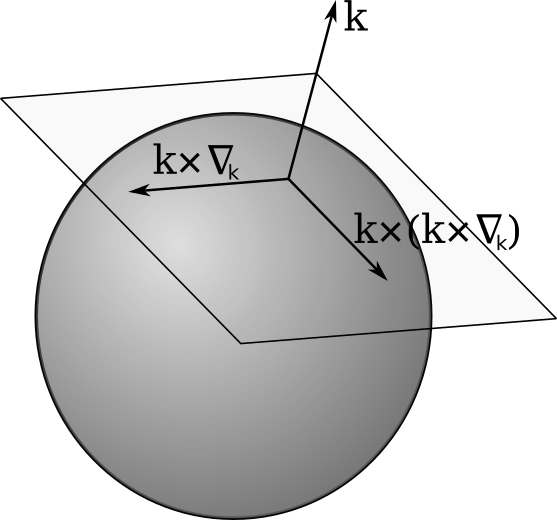
\includegraphics[scale=0.5]{vec_fourier}
\caption{Operadores vetoriais no espaço de Fourier usados para encontrar as soluções vetoriais.}
\label{vet_fourier}
\end{center}
\end{figure}
%
Obtemos, até então, os potenciais de ondas planas incidentes e espalhadas na direção $z$ em coordenadas esféricas. Queremos usa-las para montar um feixe cônico de alta abertura numérica. Faremos isso rotacionando e superpondo diversas ondas planas usando o operador ${\mathbf J}$, que é o gerador de rotações no espaço. Como a dependência angular dos potenciais de Debye estão contidas nos harmôncos esféricos, o procedimento se resume em fazer a rotação dos mesmos. Usando o operador $D(\alpha,\beta,\gamma)=e^{-i\alpha J_z}e^{-i\beta J_y}e^{-i\gamma J_z}$ e o fato de que os harmônicos esféricos são autofunções de $J_z$, obtemos:

\begin{equation}
Y_{JM}(\theta',\phi')=\sum \limits_{M'=-J}^{J} Y_{JM'}(\theta,\phi) e^{-i(\alpha M'+\gamma M)} d^J_{M'M}(\beta),
\label{harm_esf_rot}
\end{equation}
%
que representa um harmônico esférico em um eixo rodado com coordenadas $\theta'$ e $\phi'$, onde $d^{J}_{M',M}(\beta)=e^{-i\beta J_y}$ é o elemento da matriz-$d$ de Wigner e  $\alpha$, $\beta$, e $\gamma$ são os ângulos de Euler. A rotação é feita de forma que o eixo $z$ coincida com o eixo $\hat{{\mathbf k}}$ de propagação. Para isso, $\alpha =\phi_k$ e $\beta =\theta_k$. Usamos o último ângulo de Euler para determinar corretamente a direção de polarização do feixe fazendo $\gamma =-\phi_k$. Substituindo em \ref{debye_def}, os potenciais de Debye rotacionados ficam:

\begin{equation}
\Pi^E =\pm \frac{E_0 e^{-i\omega t}}{k}\sum \limits_{J=1}^{\infty}(i)^{J+1}j_J(kr)\sqrt{\frac{4\pi(2J+1)}{J(J+1)}} \sum \limits_{M'=-J}^J e^{i\phi_k(M'\mp1)}d^J_{M',\pm1}(\theta_k)Y_{JM'}(\theta,\phi),
\label{debyeE_rot}
\end{equation}
e
\begin{equation}
\Pi^M =\frac{H_0 e^{-i\omega t}}{k}\sum \limits_{J=1}^{\infty}(i)^{J}j_J(kr)\sqrt{\frac{4\pi(2J+1)}{J(J+1)}} \sum \limits_{M'=-J}^J e^{i\phi_k(M'\mp1)}d^J_{M',\pm1}(\theta_k)Y_{JM'}(\theta,\phi).
\label{debyeM_rot}
\end{equation}
%

O próximo passo é integrar no ângulo solido do cone. Começando pela varável $\phi_k$ (ou seja, componente $\phi$ da direção do vetor de onda ${\mathbf k}$; notação que será usada para $\theta_k$ também), obtemos:

\begin{equation}
\begin{split}
\Pi^E_{\theta_k} =\pm \frac{E_0 e^{-i\omega t}}{k}\sqrt{\cos(\theta_k)}\sum \limits_{J=1}^{\infty}(i)^{J+1}j_J(kr)\sqrt{\frac{4\pi(2J+1)}{J(J+1)}} \times \\ \times \sum\limits_{M'=-J}^J d^J_{M',\pm1}(\theta_k)Y_{JM'}(\theta,\phi) \int\limits_0^{2\pi} d\phi_k e^{-i\phi_k(M'\mp1)} ,
\label{pi_phi}
\end{split}
\end{equation}
%
onde o termo $\sqrt{\cos(\theta_k)}$ vem da condição do seno de Abbe. O cone sólido se obtem integrando em $\theta_k$:

\begin{equation}
\begin{split}
\Pi^E=\int\limits_0^{\theta_0}d\theta_k \sin\theta_k \Pi^E_{\theta_k}, \\
\Pi^M=\int\limits_0^{\theta_0}d\theta_k \sin\theta_k \Pi^M_{\theta_k},
\label{integral_theta}
\end{split}
\end{equation}
%
onde $\theta_0$ é a meia abertura do feixe.

Para derivar a força na microesfera em função da sua posição relativa ao foco do feixe, temos que calcular os campos deslocados em relação ao centro do objeto espalhador, ou seja, a orígem. Fazemos isso usando o gerador de translações no espaço ${\mathbf k}$, com o operador $e^{-i{\mathbf k}\cdot{\mathbf R}}$, onde ${\mathbf R}=q_x\hat{x}+q_y\hat{y}+q_z\hat{z}$ é o vetor de deslocamento. Multiplicamos esse operador em cada coeficiente de multipolo, e dessa forma, o operador fica dentro da integral em $\phi_k$, que leva ao seguinte resultado:

\begin{equation}
\begin{split}
\int\limits_0^{2\pi} d\phi_k e^{-i{\mathbf k}\cdot{\mathbf R}} e^{-i\phi_k(M'\mp1)}=e^{-ik z\thinspace \cos\theta_k} 2\pi(-i)^{M'\mp1}J_{M'\mp1}\left(k\sin\theta_k\sqrt{q_x^2+q_y^2}\right)e^{-i(M'\mp1)\phi}.
\label{int_phi}
\end{split}
\end{equation}
%

Uma vez determinados os potenciais de Debye incidentes e espalhados, podemos obter os campos aplicando os operadores $-i\nabla\times{\mathbf L}$ e $-i{\mathbf L}$:

\begin{equation}
\begin{split}
{\mathbf E}_T={\mathbf E}_{IN}+{\mathbf E}_{S}=-i\nabla\times{\mathbf L}(\Pi^E_{IN}+\Pi^E_S)+i \omega \mu(-i){\mathbf L}(\Pi^M_{IN}+\Pi^M_S), \\
{\mathbf H}_T={\mathbf H}_{IN}+{\mathbf H}_{S}=-i\nabla\times{\mathbf L}(\Pi^M_{IN}+\Pi^M_S)-i \omega \epsilon(-i){\mathbf L}(\Pi^E_{IN}+\Pi^E_S).
\end{split}
\end{equation}
%

Finalmente, calculando a integral \ref{2_F}, obtemos a força na microesfera de um campo cônico e com perfil de instensidade constante antes de entrar na objetiva. Essa integral pode ser resolvida tomando a superfície $\sigma$ como uma esfera (com centro na orígem) com raio tendendo a infinito. Isso faz com que as componentes radiais do campo sejam desprezadas no cálculo, pois caem com $\frac{1}{r^2}$, comparado às componentes tangenciais que caem com $\frac{1}{r}$. Temos, então:

\begin{equation}
{\mathbf F}=\frac{-1}{2}r\left( \int d\Omega (\epsilon E^2_{tan}{\mathbf r}) + \int d\Omega (\mu H^2_{tan}{\mathbf r}) \right),
\end{equation}
%
onde as duas integrais dentro do parentesis são iguais. Sendo assim, a força vai depender do quadrado dos campos ($E^2$ e $H^2$), e de termos proporcionais a ${\mathbf E}_{IN}\cdot{\mathbf E}_{IN}^*$(incidente-incidente), $\operatorname{Re}({\mathbf E}_{IN}\cdot{\mathbf E}_S^*)$(espalhado-incidente) e ${\mathbf E}_S\cdot{\mathbf E}_S^*$(espalhado-espalhado). O primeiro desses termos (campo incidente-incidente) não contribui para a força, pois trata-se do caso onde não há centro espalhador. O produtos dos campos espalhado-incidente é chamado termo de extinção, e representa a taxa de perda de momento do campo incidente para o centro espalhador. Por fim, o termo de espalhamento (espalhado-espalhado) é menos a taxa de transferência de momento para o campo espalhado.

A expressão para a força será mostrada depois de introduzirmos o perfil do feixe e a polarização, uma vez que tanto os campos mudam, quanto as expressões da força ganham termos adicionais. Junto com a expressão para a força, serão mostrados os coeficientes de multipolo $\G_JM$, que carregam as informações de aberrações e do perfil de intensidade.

%
%
%%%%%  Seção 2  %%%%%
%
%
\section{Efeito do perfil gaussiano}

\hspace{5 mm}O efeitos do perfil gaussiano no feixe. Faremos isso analisando o campo paraxial na entrada da obejtiva. Trataremos também do efeito da aberração esférica causada pela objetiva quando a lente é imersa em um meio com índice de refração diferente do meio que envolve a microesfera. 

Para introduzir o efeito que o perfil do feixe produz, basta saber como é o feixe paraxial antes de ser focalizado. Primeiramente, assumimos que tal feixe incidente esteja com a altura da cintura mínima coincidente com a entrada da objetiva. Isso nos permite tratar-lo como um feixe cilíndrico (de raio de curvartura infinito). {\bf colocar discussão sobre feixe paraxial em algum apendice, e fazer a referencia aqui.} O campo fica:

\begin{equation}
{\mathbf E}_{IN}^{antes}(\vec{r},t)=E_0 e^{ikz} e^{-\frac{f^2\sin^2\theta_k}{\omega_0^2}}(\hat{{\mathbf x}}\pm i\hat{{\mathbf y}}) e^{i\omega t},
\label{campo_ent}
\end{equation}
%
onde $\omega_0$ é a cintura (waist) mínima, $f^2\sin^2\theta_k=\rho^2$ (pela condição do seno) é a distância ao eixo do feixe ao quadrado. Ao passar pela objetiva, o campo também ganha uma correção de efeitos de difração \cite{1959a}, o fator multiplicativo $-i\frac{f}{\lambda}$. O fator $e^{-\frac{f^2\sin^2\theta_k}{\omega_0^2}}$ deve ser inserido dentro da integral em $\theta_k$. Assim, as expressões para os multipolos \ref{integral_theta} são alteradas.

%
%
%%%%%  Seção 3  %%%%%
%
%
\section{Efeitos de polarização}
\label{Efeitos de polarizacao}

\hspace{5 mm}Entender o caso de polarização linear vai tornar possível a compreensão do caso de polarização elíptica. Começamos modelando o feixe como uma superposição de polarização circular a direita a e esquerda, com pesos iguais. O único procedimento que muda em relação ao caso de polarização circular é quando tomamos os quadrados dos campos ${\mathbf E}$ e ${\mathbf H}$. Teremos campos espalhados e incidentes de ambas as polarizações, com as quais montamos os respectivos potenciais de Debye. Produtos de campos de mesma polarização serão chamados puros, e produtos de campos de polarização oposta serão chamados cruzados. Introduzimos, então, o fator de eficiência vetorial, também chamado de força normalizada, para o feixe de polarização linear:

\begin{equation}
{\mathbf Q} = \frac{\left<{\mathbf F}\right>}{n_1 P/c}= \frac{1}{2}{\mathbf Q}^{(\sigma +)} + \frac{1}{2}{\mathbf Q}^{(\sigma -)} + {\mathbf Q}^{({\it cross})}
\label{fatoref_forca}
\end{equation}
%
onde $\left<{\mathbf F}\right>$ é a média temporal da força e P é a potência do feixe incidente na amostra. Os termos ${\mathbf Q}^{(\sigma \pm)}$ são os termos que encontraríamos para a polarização circular direita ou esquerda (tanto de espalhamento quanto de extinção). O termo ${\mathbf Q}^{({\it cross})}$ é o que chamamos de cruzado, pois contem produtos de campos com polarizações opostas. 

A força exercida por uma polarização elípitica pode ser obtida introduzindo a dependência com o ângulo $\psi$ do eixo rápido da placa de quarto de onda (PQO, ou QWP) no feixe paraxial incidente na entrada da objetva:

\begin{equation}
{\mathbf E}^{ent}(\rho,\phi,z) = E_{centro} e^{ik_0z} e^{\frac{-\rho^2}{w_0^2}} \sum \limits_{\sigma = +1,-1} \frac{1 - ie^{-2i\sigma \psi}}{2} \hat{\bf{\epsilon}}_\sigma .
\label{l}
\end{equation}
%
Dessa forma, os potenciais de Debye ganham um termo a mais devido ao ângulo da placa de quarto de onda. Podemos, então, identificar 4 tipos de termos nas forças de extinção e de espalhamento: diretos ou puros devidos as polarizações $\sigma_\pm$, e termos cruzados com os produtos $\sigma_\pm^*\cdot\sigma_\mp$.

%
%
%%%%%  Seção 4  %%%%%
%
%
\section{Aberração esférica produzida por refração na interface com o porta-amostra}
\label{Aberracao esferica}

\hspace{5 mm}A aberração esférica é um efeito ótico onde os raios que compõem o feixe são focalizados em pontos distintos do eixo ótico. Uma lente esférica, por exemplo, fará com que os raios marginais de um feixe colimado sejam mais refratados que os raios mais próximos ao eixo ótico. Esse efeito faz com que o perfil de intensidade do feixe seja difundido ao longo do eixo ótico.

{\bf Antes mesmo do feixe ser focalizado, este pode conter aberração esférica, como veremos na próxima seção.}

Uma outra forma que a aberração esférica pode ocorrer é quando há algum tipo de feixe focalizado atravessando a interface de meios com índices de refração diferentes. Nesse caso, é fácil de mostrar como o efeito funciona em uma abordagem de ótica de raios e a lei de Snell. Componentes do feixe no meio com índice $n$ que incidem na interface com ângulo $\theta$, por refração, são transmitidos com um ângulo $\theta_1$ no meio com índice de refração $n_1$, de forma a respeitar a lei de Snell:
%
\begin{equation}
n\sin\theta=n_1\sin\theta_1.
\label{snell}
\end{equation}
%

Fica claro, então, que para um feixe focalizado incidindo com seu eixo perpendicular à interface, raios que incidem em direções com ângulo $\theta\ne 0$, ao mudarem de meio, não mais incidem no foco. Portanto, a região de maior intensidade não se localiza mais no ponto focal, e sim difundida e mais próxima à interface. No aparato de pinças óticas esse efeito ocorre quando usamos uma lente objetiva de imersão em óleo, que não é corrigida para aberração esférica, e o feixe incidide em um porta-amostra contendo algum fluido com índice de refração diferente do óleo e do vídro do porta-amostra, que são iguais. Esse efeito faz com que a posição de equilíbro da microesfera se desloque para mais perto da interface.
%
\begin{figure}
\begin{center}
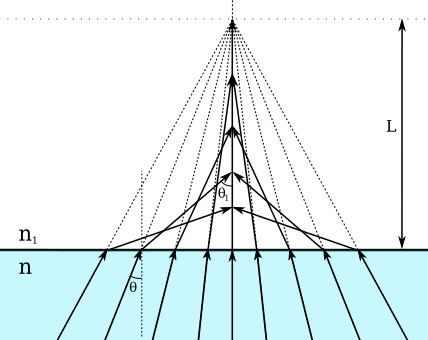
\includegraphics[scale=1.]{aberracao_esf}
\caption{}
\label{ab_esf}
\end{center}
\end{figure}
%

Podemos entender esse efeito também como uma diferença de caminho ótico induzida no feixe. Esta 

Ao serem refratadas, as componetes de onda-plana ganham também uma fase $e^{i\Psi(z, \theta)}$, onde

\begin{equation}
\Psi(z,\theta)=k\left( -\frac{L}{N^2}\cos\theta +(L+z)\cos\theta_1 \right) 
\label{faseSA}
\end{equation}
%
é a função de aberração esférica.

Para modelar a passagem de um meio para outro, levamos em conta a amplitude de transmissão de Fresnel de cada componente ${\mathbf k}$ do campo, dada por \cite{Viana2007}:

\begin{equation}
T(\theta)=\frac{2\cos\theta}{\cos\theta + N\cos\theta_1} ,
\label{transmitancia}
\end{equation}
%
onde, por \ref{snell}, $\theta_1=\arcsin(\frac{\sin\theta}{N})$. 

%
%
%%%%%  Seção 5  %%%%%
%
%
\section{Aberrações óticas}

\hspace{5 mm}As aberrações óticas são modificações nos feixes paraxiais induzidas por uma série de fatores, entre eles imperfeições nas lentes e desalinhamentos no sistema ótico. O estudo das aberrações é inspirado pelo fato de que a teoria MDSA subestima a força radial na pinça ótica quando o raio da microesfera aprisionada é menor ou da ordem do comprimento de onda $\lambda$ do laser\cite{Dutra2014}. Raios maiores que $\lambda$ recuperam tanto os resultados da teoria MDSA quanto os da ótica geométrica. Isso ocorre porque a esfera passa a sondar uma média do perfil do feixe, em contraste com o caso anterior, em que ela sonda diferenças de fase e distribuição de intensidade do feixe focalizado.

O formalismo de Seidel é um dos possíveis métodos para se descrever as aberrações em um feixe paraxial. Entre as aberrações primárias, que aparecem como os primeiros termos de uma expansão nesse formalismo, são relevantes para o nosso modelo o astigmatismo, a coma e a aberração esférica \cite{Dutra2014}. Estamos tratando aqui de aberrações antes da objetiva, ou seja, a aberração esférica tratada aqui tem orígem diferente da descrita na sessão anterior, apesar de serem o mesmo fenômeno físico.

Podemos introduzir essas aberrações no modelo colocando a fase adicional $e^{i\Phi_{adicional}(\theta,\phi)}$ nos campos na entrada da objetiva (modificando a equação \ref{l}), com:

\begin{equation}
\Phi_{adicional}(\theta,\phi) = 2\pi \left[ A'_{sa}\left( \frac{\sin\theta}{\sin\theta_0} \right)^4 + A'_{c}\left( \frac{\sin\theta}{\sin\theta_0} \right)^3\cos(\phi - \varphi_c) + A'_{a}\left( \frac{\sin\theta}{\sin\theta_0} \right)^2\cos^2(\phi - \varphi_a) \right].
\end{equation}
{\bf atenção aqui! tese do Rafael$->$ cos do $A_{ast}$ é diferente (2(angulo), elevado ao quad), no artigo do Kaina, essa fase é referida como fase de Zernike, e tirei da tese do Rafa como fase de Seidel. }
%
Identificamos $A'_{sa}$, $A'_{c}$ e $A'_{a}$ como os parâmetros de aberração esférica ($sa$ do inglês, {\it spherical aberration}), coma e astigmatismo. Para entender os parâmetros $\varphi_c$ e $\varphi_a$, temos que entender o que são essas aberrações. A primeira característica delas é a quebra de simetria no plano perpendicular a propagação do feixe paraxial (eixo $z$), e os parâmetros $\varphi_c$ e $\varphi_a$ são os eixos da orientação dos efeitos de coma e astigmatismo respectivamente. Isso também explica o porquê de não haver um parâmetro angular para aberração esférica: trata-se de uma aberração simétrica em $\phi$, o que fica muito claro pela seção anterior.
%
\begin{figure}[h]
\begin{center}
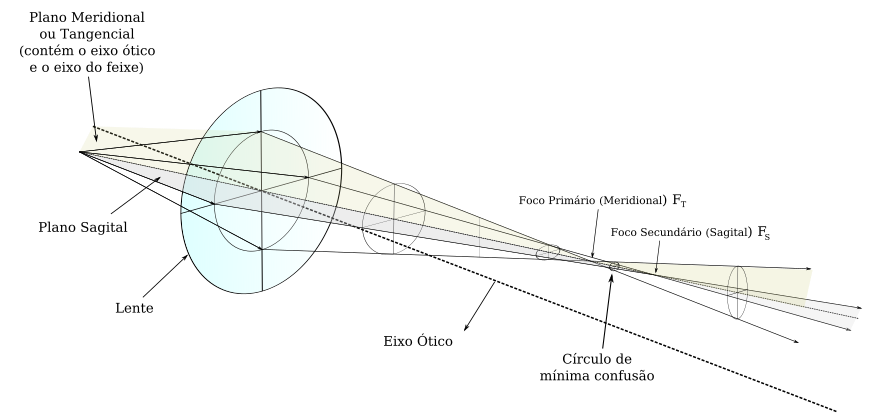
\includegraphics[scale=.7]{feixe_astig}
\caption{Feixe com astigmatismo.}
\label{feixe_astig}
\end{center}
\end{figure}
%

Uma breve explicação das aberrações será feita a seguir, baseada em trabalhos do grupo \cite{Dutra, Diniz2019, Dutra2014}, onde detalhes do seguinte desenvolvimento podem ser encontrados. 

Considemos agora o problema prático: os experimentos que serviram de base comparatória para as simulações desenvolvidas não possuem coma e os efeitos de aberração esférica podem ser negligenciados. Portanto, somente o astigmatismo será levado em conta nas equações apresentadas. Como a fase referente ao astigmatismo possui uma dependência em $\phi$, podemos concluir que a integral da equação \ref{int_phi} será modificada. 

Uma vez apresentadas todas as correções feitas ao modelo MD, vamos apresentar as expressões para força em termos dos coeficientes de multipolo.

%
%
%%%%%  Seção 6  %%%%%
%
%
\section{Força ótica em termos da expansão em multipolos}
\label{forcaotica}

\hspace{5 mm}Como apresentado no começo do capítulo, o método para se obter a força na pinça ótica é resolver a integral \ref{2_F}. A forma mais fácil de faze-lo é tomando a superfície $\sigma$ no infinito, já que a escolha dessa é arbitrária. Podemos argumentar também que a integral envolvendo o vetor de Poynting é zero. No limite que tal superfície está no infinito, usamos as expressões assintóticas das funções de Bessel (com dependência em $kr$) dentro dos potenciais de Debye. 

Portanto, a expressão para as contribuições de espalhamento e extinção do fator de eficiência na direção $z$, para uma polarização qualquer, corrigida para aberração esférica e astigmatismo, tem a forma \cite{Diniz2019}:

\begin{equation}
\begin{split}
Q_{sz}(\rho,\phi,z) = -\frac{4\gamma^2}{AN}\operatorname{Re}\sum\limits_{jm\sigma} \Big{[} \frac{\sqrt{j(j+2)(j+m+1)(j-m+1)}}{j+1} \Big{(} (a_ja^*_{j+1}+b_jb^*_{j+1})\times \\ \G^{(\sigma)}_{j,m}\G^{(\sigma)*}_{j+1,m}(1-\sigma\sin2\psi) + (a_ja^*_{j+1}-b_jb^*_{j+1})\G^{(\sigma)}_{j,m}\G^{(-\sigma)*}_{j+1,m}\cos2\psi e^{i2\sigma(\phi-\psi)} \Big{)} + \\ \frac{2j+1}{j(j+1)} m\sigma a_jb^*_j\big{(} |\G^{(\sigma)}_{j,m}|^2(1-\sigma\sin2\psi)-\G^{(\sigma)}_{j,m}\G^{(-\sigma)*}_{j,m}\cos2\psi e^{i2\sigma(\phi-\psi)} \big{)} \Big{]},
\end{split}
\end{equation}
%
\begin{equation}
Q_{ez}(\rho,\phi,z) = \frac{2\gamma^2}{AN}\operatorname{Re}\sum\limits_{jm\sigma} (2j+1)\G^{(\sigma)}_{j,m} \Big{[} (a_j+b_j) \G^{C,(\sigma)*}_{j,m}(1-\sigma\sin 2\psi) + (a_j-b_j) \G^{C,(-\sigma)*}_{j,m}\cos2\psi e^{i2\sigma(\phi-\psi)} \big{]}.
\end{equation}
%

O fator $\gamma=f/\omega_0$ é a razão entre a distância focal e a cintura do feixe na entrada da objetiva, enquanto o fator $A$, denominado {\it filling factor}, é a fração de potência que é transmitida pela objetiva. Deixamos para o apêndice \ref{apendicea} as expressões para os coeficiente de multipolo $\G^{(\sigma)}_{j,m}$ e $\G^{C,(\sigma)}_{j,m}$, além das expressões para as componentes radiais e azimutais do fator de eficiência $Q_\rho$ e $Q_\phi$, e dos multipolos $\G^{\pm,(\sigma)}_{j,m}$ dos quais os dois últimos dependem.

No capítulo \ref{cap3} serão descritas as medidas feitas com o aparato da pinça ótica. As forças não são medidas diretamente: como as microesferas estão em movimento browniano na solução, quando pinçadas elas passam flutuar ao redor da posição de equilíbrio na pinça. Seus movimento pode ser descrito por meio de um potencial harmônico, que permite uma expansão de Taylor da força em $\rho$, e uma constante elástica associada a pinça. Temos, então, a constante transversa $\kappa_\rho$ de rigidez dada por\cite{Viana2007}:
%
\begin{equation}
\kappa_\rho=-\frac{n_1 P}{c}\frac{\partial Q_\rho}{\partial \rho}\Big{|}_{\rho=0, \thinspace z=z_{eq}},
\label{kphi}
\end{equation}
%
onde $P$ é a potência do laser; e a constante de torção \cite{Diniz2019}:
%
\begin{equation}
\kappa_\phi=-\frac{n_1 P}{c}\frac{\partial Q_\phi}{\partial \rho}\Big{|}_{\rho=0, \thinspace z=z_{eq}}.
\label{kphi}
\end{equation}
%

Os somatórios em $j$ e $m$ são feitos da mesma forma que na expressão \ref{pi_phi}: $j$ vai de $0$ a $\infty$, e $m$ de $-j$ a $j$. Os valores da soma de $\sigma$ são $\pm1$, como na equação \ref{l}. O importante de observarmos aqui é a dependência de $Q_z$ com $\psi$, que será um parâmtero livre no experimento e portanto na simulação. Podemos identificar nas expressões 4 tipos de termos: com multipolos com mesmo índice de polarização $\G^{(+1)}\G^{(+1)*}$ e $\G^{(-1)}\G^{(-1)*}$, e com índices invertidos $\G^{(+1)}\G^{(-1)*}$ e $\G^{(-1)}\G^{(+1)*}$. Os dois primeiros termos são proporciais, respectivamente, a $(1-\sin2\psi)$ e $(1+\sin2\psi)$, e os dois últimos, a $\cos2\psi e^{i2\psi}$ e $\cos2\psi e^{-i2\psi}$.

Explicitar essa soma é de grande importância para os cálculos numéricos, pois podemos calcular esses 4 termos de forma independente, e teremos o valor de $Q_z$ para qualquer ângulo da placa de quarto de onda.

\section{Interação Spin-Órbita}
\label{interacao_so}

\hspace{5 mm}Uma das características da pinça ótica que faz com que a modelagem teórica seja tão difícil é o fato de que o feixe que emerge da objetiva é muito focalizado, e portanto não paraxial. Um dos efeitos resultantes da focalização do feixe é a conversão de momento angular de spin do feixe, associado a polarização (ou helicidade) do campo, em momento angular orbital \cite{Bliokh2015}. O momento angular orbital insere uma fase com dependência na variável cilindrica $\phi$.

Evidências experimentais apontam que o campo espalhado por uma microesfera no aparato de pinça ótica pode carregar mais momento angular do que o campo incidente. Usamos o efeito de conversão de momento angular de spin para orbital junto com a teoria MD para pinça ótica para trazer luz a esse fenômeno.

De uma forma simples, podemos entender essa transferência de momento angular considerando um cone de ondas planas circularmente polarizdas com angulo de meia abertura $\theta$, da mesma forma que fizemos no começo da seção \ref{MD}. 

Suas componentes de spin apontam para as respectivas direções de propagação, com o sentido definido pelo sentido da polarização circular {\bf colocar referência}. Assumindo que o momento angular (intrínsico) total se conserve, vemos que a soma dos vetores diametralmente opostos terão suas componentes radiais se anulando, enquando as na direção axial se somam. Se ${\mathbf P}$ é o momento angular total do feixe e ${\mathbf S}$ e ${\mathbf L}$ são os momentos angulares de spin e orbital, temos a seguinte relação \cite{Bliokh2015}:
%
\begin{equation}
{\mathbf S}=\sigma\cos\theta{\mathbf P}\thinspace, \quad\quad {\mathbf L}=\sigma(1-\cos\theta){\mathbf P}.
\end{equation}
%

Na seção \ref{MD} rotacionamos os potenciais de Debye, que representam ondas paciais, utilizando um operador de rotação. Podemos, ao invés disso, rotacionar o campo vetorial ${\mathbf E}$ diretamente. Essa rotação pode ser representada na base de polarização circular $\ket{\sigma +}$, $\ket{\sigma -}$ e $\ket{z}$ com a seguinte transformação unitária \cite{Bliokh2011}:
%
\begin{equation}
\begin{pmatrix}
\braket{\sigma+|E'} \\
\braket{\sigma-|E'} \\
\braket{z|E'} 
\end{pmatrix}
=
\begin{pmatrix}
a & be^{-i2\phi} & \sqrt{2ab}e^{-i\phi} \\
-be^{i2\phi} & a & \sqrt{2ab}e^{i\phi} \\
-\sqrt{2ab}e^{i\phi} & -\sqrt{2ab}e^{-i\phi} & a-b
\end{pmatrix}
\begin{pmatrix}
\braket{\sigma+|E} \\
\braket{\sigma-|E} \\
\braket{z|E} 
\end{pmatrix}.
\end{equation}
%
A dependência com o ângulo $\phi$ também aparece nas expressões dos campos rotacionados (equação \ref{pi_phi}), ao rotacionarmos os harmônicos esféricos (equação \ref{harm_esf_rot}) com $\alpha=-\gamma=\phi_k$.

Uma vez que haja momento angular orbital incidindo na microesfera, podemos fazer um paralelo com a transferência de momento linear para explicar o excesso de momento angular no campo espalhado.

Como discutido na seção \ref{MD}, os termos de extinção representa a quantidade de momento que é transferida do campo incidente à microesfera; enquanto o termo de espalhamento está relacionado à transferência de momento para o campo espalhado. Podemos entender que, na região de pequenos raios, o termo que domina na expressão da força é o de extinção, pois se o raio da esfera é muito menor que o comprimento de onda do laser, pode-se concluir que o campo não será tão afetado por esse centro espalhador (${\mathbf E}_S$ é muito pequeno e $\operatorname{Re}({\mathbf E}_{IN}\cdot{\mathbf E}_S^*)$ domina sobre ${\mathbf E}_S\cdot{\mathbf E}_S^*$). 

Quanto maior for o centro espalhador, mais afetado o campo será, e a partir de um certo raio, o termo de espalhamento da força domina \cite{}{\bf encontrar referência}. A imagem \ref{Kphi_raio} mostra o comportamento da constante de torção $\kappa_\phi$.
%
\begin{figure}[h]
\begin{center}
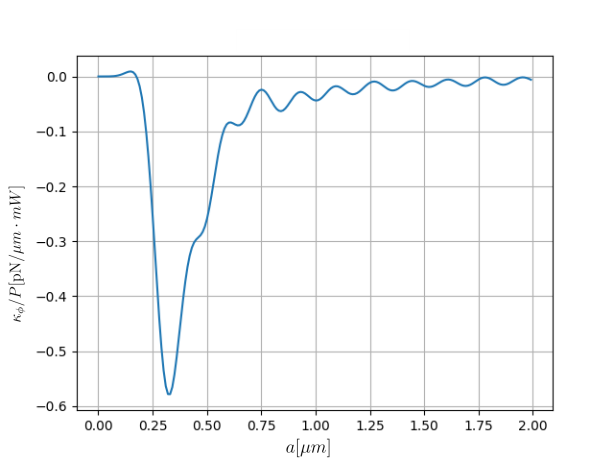
\includegraphics[scale=.85]{Kphi_Artigo_Kaina}
\caption{Constante de torção $\kappa_\phi$ em função do raio da microesfera. O comprimento de onda do laser é de $1064 nm$, a distância $L$ entre o foco e a lamínula é de $4,5$ unidades de raio e a polarização $\sigma+$. Astigmatismo não é levado em conta nessa simulação.\\{\bf colocar informações sobre os dados (comp de onda, aberração esferica, ausencia de astig, polarização, etc.).}}
\label{Kphi_raio}
\end{center}
\end{figure}
%

Podemos observar que na região em que o raio $a$ é menor que $0,15 \mu m$, a constante de torção é positiva, e o torque indica um ganho de momento angular na mesma direção ao de spin do campo incidente. Sendo essa a região onde o termo de extinção domina, podemos inferir que o campo está cedendo momento angular para a microesfera, e esta não está espalhando momento angular o suficiente para sofrer torque negativo.


Quando o raio aumenta, a componente de espalhamento da força começa a dominar, e efeitos de torque negativos a prevalecer. Podemos concluir que o campo espalhado carrega momento angular em excesso. Como a componente de spin do campo espalhado não podem ser maior que do incidente, por esta última já ser máxima, o excesso de momento angular tem que ser de origem orbital. 

\end{chapter}